\quad \quad In this chapter, we will look at composition of functions and inverse functions. You can use the normal arithmetic operations on functions like how you would to numbers:

\begin{example}
  If \(x=2\) and \(f(x)=x^2+4\):
  \begin{equation*}
    f(x)+f(x) = 2^2+4+2^2+4=16 
  \end{equation*}
  \begin{equation*}
    \frac{f(x)}{2} = \frac{2^2+4}{2} = 4 
  \end{equation*}
\end{example}

What is more interesting, perhaps, is taking the \textit{output} of a function and use it as the \textit{input} to another function. You may also think of it as "piping" one function into another. This is called \textit{function composition}.


  \begin{figure}[h]
  \centering
  \marginnote{\footnotesize \textit{Note that the rectangles are \\ functions and circles are values.}}
  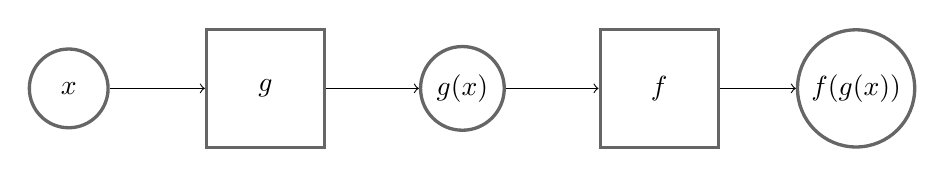
\begin{tikzpicture}[
roundnode/.style={circle, draw=black!60, fill=white!5, very thick, minimum size=10mm},
squarednode/.style={rectangle, draw=black!60, fill=white!5, very thick, minimum size=15mm},
]
    \node[roundnode] (x) {\(x\)};
    \node[squarednode] (maintopic) [right of=x, xshift=1.5cm] {\(g\)};
    \node[roundnode] (fx) [right of=maintopic, xshift=1.5cm] {\(g(x)\)};
    \node[squarednode] (gtopic) [right of=fx, xshift=1.5cm] {\(f\)};
    \node[roundnode] (final) [right of=gtopic, xshift=1.5cm] {\(f(g(x))\)};
    \draw[->] (maintopic.east) -- (fx.west);
    \draw[->] (x.east) -- (maintopic.west);
    \draw[->] (fx.east) -- (gtopic.west);
    \draw[->] (gtopic.east) -- (final.west);
  \end{tikzpicture}
  \caption{Visual representation of function composition.}

\end{figure} 

Another notation for composing functions together(which we will not really use) is as such:
\begin{equation*}
  f(g(x))=(f \circ g)(x) 
\end{equation*}

When you compose the same function \(n\)-times, the notation for it is:
\begin{equation*}
f^n(x)=\underbrace{f(f(\ldots f(x)))}_{n-times} 
\marginnote{\footnotesize \textit{However, this does not \\ apply to trigonometric functions. \(sin^2(x)\) is \(sin(x) \times sin(x)\) instead of \(sin(sin(x))\) and \(sin^{-1}(x)\) is \(arcsin(x)\).}}
\end{equation*}
\newpage
\begin{example}
  Here are some examples of composing functions together:
  If \(x=3\) and \(f(x)=\pi x\), \(g(x)=sin(x)+1\):
  \begin{equation}
    g(f(x))=sin(\pi \times 3)+1=1 
  \end{equation}
  \begin{equation}
    f^3(x)=\pi^{3}x 
  \end{equation}
  \quad \, There is nothing much here, really, just evaluate the function from the innermost function to the outermost.
\end{example}
\begin{theorem}
  Given functions \(f:X \to Y\), \(g: Y \to Z\) and \(h: Z \to W\), prove that the composition of the three functions is \textit{associative}, in other words:
  \begin{equation*}
    h \circ (g \circ f) = (h \circ g) \circ f
  \end{equation*}
\end{theorem}
\begin{proof}
  Let \(x \in X\), we have: 
  \begin{equation*}
    h \circ (g \circ f(x)) = h(g \circ f(x)) = h(g(f(x))) = h \circ g(f(x)) = (h \circ g)f(x)
  \end{equation*}
  This proves the associativity of function composition.
\end{proof}
\begin{remark}
  This is just a fun little exercise for the reader and ultimately is not that important to the entire book, just a good identity to keep in the back of your mind. 
\end{remark}

Next, we will delve into inverse functions. Let us start with one I believe you may have seen before, look at the following figure: 
\begin{figure}[h]
  \centering
  \begin{tikzpicture}[scale=1.8]
        \coordinate (a) at (0,0);
        \coordinate (b) at (4,0);
        \coordinate (c) at (4,2);
        \draw (a) -- (b)node[midway, below]{a} -- (c)node[midway,right]{b} -- (a)node[midway,left, above]{c}; % Triangle.
        \draw (a) node[anchor=east,align=center] {B};
        \draw (b) node[anchor=west,align=center] {C};
        \draw (c) node[anchor=south]{A};
        \MarkRightAngle{a}{b}{c}; 
\end{tikzpicture}
\caption{Figure of right triangle ABC.}
\end{figure}

If I ask you what is \(arcsin(B)\), you may say it is \(\frac{b}{c}\). But, what is \(arcsin(sin(B))\), well, that is just \(B\), isn't it. Hence, the \(arcsin\) sort of "cancels" the \(sin\). We call \(arcsin\) the \textit{inverse function} or just inverse of \(sin\). 
